\section{Model of the Caches}
\label{sec:model:cache}
This section presents the automaton that corresponds to a cache.

This is where the table defining the cache's behavior in the cache coherence
protocol description is implemented. However, this table corresponds to the
cache's behavior for a single memory element, whereas the cache has to handle
a great number of them. As a result, the automaton presented in this section
does not resemble the one described in a cache coherence protocol table.
\iffalse
Instead, the behavior described by the table is implemented by the automaton's
transitions, but the coherence states are stored within a local variable array.
\fi
In effect, the transitions of this automaton are focused on what corresponds to
events in the table, and actions that lead to such events being emitted.

\begin{figure}[hbt!]
\begin{center}
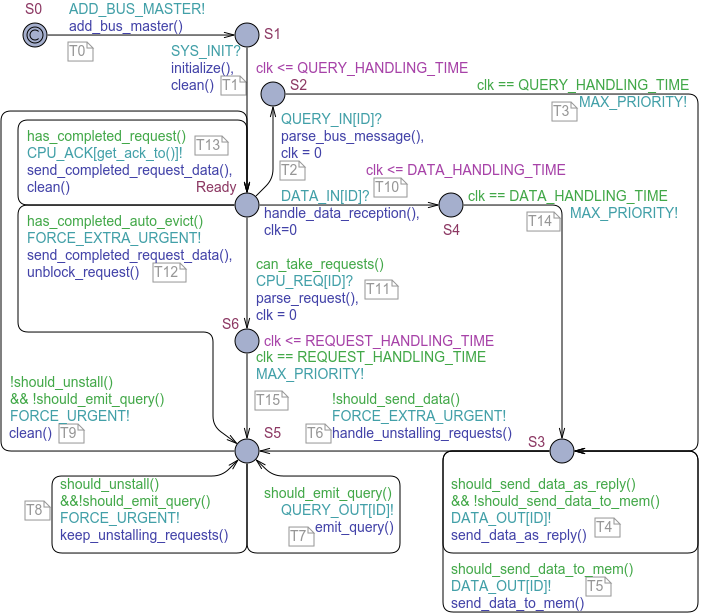
\includegraphics[width=\textwidth]{\chapterdirectory/figure/MSICacheCTRL.pdf}
\end{center}
\caption{Automaton for a Cache}
\label{fig:UPPAAL:MSICacheCTRL}
\end{figure}

Figure~\ref{fig:UPPAAL:MSICacheCTRL} shows the automaton corresponding to a
cache. This is by far the most complex automaton in the model.

\subsection{Initialization}
Cache automata feature the following clock:
\paragraph{Clocks \& Variables for Cache Initialization}
\begin{itemize}
\item
   \lstinline!clk! is a clock used to manage times during which the cache
   automaton is to be considered inactive.
\end{itemize}
%\end{varandclocks}

The automaton starts in the $S_0$ location.

\paragraph{Transitions for Cache Initialization}
\begin{description}
\item[$S_0 \automatatransitiontrace{T_0}{} S_1$]
   The automaton starts by synchronizing with the query bus on the
   \textbf{ADD\_BUS\_MASTER} in order to be added to the list of components that
   can emit queries on that bus. This uses the information transmission shared
   variable in order to communicate to the other automaton the component ID of
   this cache. After this, the automaton enters the $S_1$ location in order to
   wait the \textbf{SYS\_INIT} broadcast.

\item[$S_1 \automatatransitiontrace{T_1}{} \texttt{Ready}$]
   Upon synchronization on the \textbf{SYS\_INIT} channel, the automaton sets
   all its internal variables to sane default values. For example, all cache
   lines are set to the \textit{Invalid} state. Each cache line has its
   \lstinline!last_use! value set to its index in the cache lines array.
\end{description}

\subsection{Cache Lines}
In cache automata, cache lines are modeled using the following variables:
\paragraph{Clocks \& Variables for Cache Lines}
\begin{itemize}
\item
   \lstinline!cache_lines! is an array of \lstinline!LINES_PER_CACHE!
   elements containing the information pertinent to every cache line (see
   Definition~\ref{def:cache_line_model}).
\item
   \lstinline!current_line! is the index of the cache line relevant to whatever
   operation is in progress. Thus, the line only needs to be found once, and its
   index can be used across multiple transitions of the automaton.
\end{itemize}
%\end{varandclocks}
These two variables are used in just about every function of the automaton, as
they are, in effect, modeling the cache's current state.

\begin{definition}[Cache Line Model]
\label{def:cache_line_model}
Caches lines are defined as $\langle \texttt{addr}, \texttt{c\_state},
\texttt{last\_use}, \texttt{reply\_to} \rangle$ tuples, with \texttt{addr}
corresponding to the address of the memory element being held, \texttt{c\_state}
its coherence state (including transient states), \texttt{last\_use} indicating
how many lines were accessed more recently than this one, and \texttt{reply\_to}
being the identifier of a cache ($\replytofun{}$ from
Definition~\ref{def:cache_info}, Chapter~\ref{cha:cache_coherence}).
\end{definition}
\begin{example}[Cache Line Model]
A cache line with a value of $\langle 91, \text{MODIFIED}, 31, 3 \rangle$
corresponds to a copy of the memory element $91$, in the \textit{Modified}
state. 31 cache lines have been accessed since this one was last accessed. The
cache with component ID 3 has been associated with this memory element.
\end{example}

Caches frequently have to find the cache line corresponding to a particular
memory element. This is done either to consult the current state of the memory
element in this state, or to change it to a new one. The cache line index
returned when trying to find a memory element corresponds to either:
\begin{itemize}
\item The cache line currently holding the targeted memory element.
\item
   The first cache line for which the coherence state is \lstinline!INVALID!,
   if the targeted memory element is not held by the cache.
\item
   A special value (\lstinline!-1!) if the  targeted memory element is not held
   by the cache, and there is no cache line in the \lstinline!INVALID! state.
\end{itemize}
When attempting to consult the current state of the targeted memory element,
that last case will be considered to yield \lstinline!INVALID!, since the memory
element is not in the cache. When attempting to change the state
associated with the targeted memory element however, having neither the memory
element nor any cache line in the \lstinline!INVALID! state means that a cache
line has to be evicted. This thus triggers the LRU eviction policy.
\iffalse
\lstset{%
   escapeinside={(*}{*)},%
   keywordstyle=\bfseries,%
   morekeywords={while,let,in,if,then,else,def,foreach},%
   numbers=none%
}
\begin{lstlisting}
result (*$\gets$*) -1
i (*$\gets$*) 0
while (i < LINES_PER_CACHE)
   if (cache_line[i].addr == TARGET)
      result (*$\gets$*) i
      break
   if ((result == -1) && (cache_line[i].c_state == INVALID))
      result (*$\gets$*) i
   i (*$\gets$*) i + 1
\end{lstlisting}
\fi

\subsection{Modeling the LRU policy}
The LRU policy uses this local variable from the cache automata:
\paragraph{Clocks \& Variables for Cache Replacement Policy}
\begin{itemize}
\item
   \lstinline!least_recently_used_line! keeps track of the least recently
   used cache line's index. This variable is used whenever an automated
   eviction occurs (and those are triggered by \lstinline!parse_request()!),
   and updated whenever an access is made to a cache line (which is the case in
   \lstinline!parse_request()! and the unstalling functions).
\end{itemize}
%\end{varandclocks}

\begin{definition}[Cache Line Access]
A cache line is considered to be accessed when either a \storeinstr{} or a
\loadinstr{} request is applied to it. Thus, \evictinstr{} is not counted as an
access.
\end{definition}

As indicated in Definition~\ref{def:cache_line_model}, each cache line has an
integer corresponding to the number of cache lines that were accessed since it
itself was last accessed. To maintain this, any access to a cache line leads
to the algorithm shown in Figure~\ref{fig:UPPAAL:lru_algo} being executed.

\begin{figure}[hbt!]
\lstset{%
   escapeinside={(*}{*)},%
   keywordstyle=\bfseries,%
   morekeywords={while,let,in,if,then,else,def,foreach},%
   numbers=none%
}
\begin{lstlisting}
threshold (*$\gets$*) cache_lines[line_being_used].last_use
i (*$\gets$*) 0
while (i < LINES_PER_CACHE)
   if (cache_lines[i].last_use < threshold)
      cache_lines[i].last_use (*$\gets$*) cache_lines[i].last_use + 1
   if ((cache_lines[i].last_use == (LINES_PER_CACHE - 1)) && (i != line_being_used))
      least_recently_used_line (*$\gets$*) i
   cache_lines[line_being_used].last_use (*$\gets$*) 0
\end{lstlisting}
\caption{LRU Algorithm}
\label{fig:UPPAAL:lru_algo}
\end{figure}

In effect, cache lines that were already less recently used than the line
currently being accessed are untouched. The cache lines that were more recently
used have their \lstinline!last_use! value incremented by one, while the one
being accessed has it set to zero. This does indeed ensure that
\lstinline!last_use! still indicates how many cache lines were accessed since
the one at \lstinline!line_being_used! was accessed.

\subsection{Handling Requests}
\label{sec:model:cache:requests}
The handling of requests is managed using the following local variables:
\paragraph{Clocks \& Variables for Request Handling}
\begin{itemize}
\item
   \lstinline!pending_requests! is an array of \lstinline!REQ_BUFFER_SIZE!
   pending requests (see Definition~\ref{def:pending_request_model}). It
   corresponds to requests from cores that have not been fully completed yet.
   It may also hold an automatically generated \evictinstr{} request.
\item
   \lstinline!completed_requests! is another array of
   \lstinline!REQ_BUFFER_SIZE! pending requests. This time, it corresponds to
   requests that are already completed, but for which acknowledgment has yet to
   be given.
\item
   \lstinline!blocked_request! is a pending request. This variable is used
   whenever an incoming request requires the replacement policy to evict a cache
   line. In such cases, \lstinline!blocked_request! is set to value of the new
   request, and an \evictinstr{} for the \lstinline!least_recently_used_line! is
   handled instead, the \lstinline!blocked_request! being considered only after
   that \evictinstr{} completes.
\item
   \lstinline!current_request! keeps track of the index of the element from
   \lstinline!pending_requests! being handled.
\item
   \lstinline!current_query! is a variable containing the data for a query to send
   out.
\end{itemize}
%\end{varandclocks}

\begin{definition}[Pending Request Model]
\label{def:pending_request_model}
Pending requests are defined as $\langle \texttt{requester}, \texttt{addr},
\texttt{cmd}\rangle$ tuples, with \texttt{requester} being the identifier of
the component that made the request, \texttt{addr} being the memory element
targeted, and \texttt{cmd} being the instruction to apply.
\end{definition}
\begin{example}[Pending Request Model]
A pending request with a value of $\langle 3, 91, \loadinstr{} \rangle$
corresponds to a request from the component of ID $3$ making a \loadinstr{} on
the memory element $91$.
\end{example}

\paragraph{Transitions for Request Handling}
\begin{description}
\item[$\texttt{Ready} \automatatransitiontrace{T_{11}}{} S_6$] The $T_{11}$
   transition corresponds to the reception of a request from a core. The request
   is obtained by synchronizing on the \textbf{CPU\_REQ} sub-channel
   corresponding to the cache's identifier. For this transition to be allowed,
   the \lstinline!pending_requests! must have at least two free slots. The extra
   slot is required in case an automatic eviction must be added to the array.
   Reception of a request makes the cache unavailable for a small amount of
   time, hence \lstinline!clk! being set to zero.

   Upon reception of the request, the cache line corresponding to the relevant
   memory element is located. If no cache line is available, the request is put
   into \lstinline!blocked_request! and the execution continues as if the new
   request had been an \evictinstr{} emitted by this very cache for the memory
   element held in the \lstinline!least_recently_used_line! cache line.

   The \lstinline!addr! of the cache line that was chosen is set to the address
   targeted by the request. This ensure that if it was an unused cache line, the
   stored address is the right one.

   The actions then performed as those indicated by the cache protocol for the
   reception of a request of that type, on a memory element with the coherence
   state currently held in the identified cache line (see
   Section~\ref{sec:modeling:precise_cache_actions} for more details). If the
   actions do not include a \hitact{}, the request is then added to the
   \lstinline!pending_requests! array as if in a queue. Otherwise, the \hitact{}
   will have added it to the \lstinline!completed_requests! array.

\item[$S_6 \automatatransitiontrace{T_{15}}{} S_5$]
   The cache becomes active after having waited the
   \lstinline!REQUEST_HANDLING_TIME! delay caused by the reception of a demand
   from the core, and is now able to complete the handling of the new request.

\item[$S_5 \automatatransitiontrace{T_{7}}{} S_5$]
   If the request being handled had an action that required it to send a query
   (\lstinline!current_query! targets a memory element other than
   \lstinline!NULL!), the sending is done by this transition. It synchronizes on
   the \textbf{QUERY\_OUT} sub-channel corresponding to this cache's identifier
   in order to communicate the query in \lstinline!current_query! to the cache's
   query FIFO automaton.

\item[$S_5 \automatatransitiontrace{T_{8}}{} S_5$]
   If no query have to be sent because of the handled request, all actions for
   this request that needed to be done at this point have been done. However,
   if the state of the targeted memory element has changed, there may be some
   older pending request for that memory element that could be un-stalled. If
   this older request has actions other than \stallact{} when the memory
   element is in its current coherency state, then that older request becomes
   the current request and those actions are applied (here also, the actions
   are described in Section~\ref{sec:modeling:precise_cache_actions}). If this
   is not the case, the current request is unchanged, and the $T_9$ transition
   is ready to be taken.

\item[$S_5 \automatatransitiontrace{T_{9}}{} \texttt{Ready}$]
   If neither the $T_7$ transition nor the $T_8$ one can be taken, the $T_9$
   transition simply resets all the internal variables that were used to quickly
   access whatever array line was relevant (e.g. \lstinline!current_line!).
   The cache automaton is then able to return to its \texttt{Ready} state.

\item[$\texttt{Ready} \automatatransitiontrace{T_{13}}{} \texttt{Ready}$]
   If there is an element in the \lstinline!completed_requests! array, whose
   \texttt{requestor} ID is not that of this cache, a synchronization on the
   \textbf{CPU\_ACK} sub-channel of the \texttt{requestor} is used to inform of
   the completion of a request. The information transmission shared variable is
   set to contain the request, although this information is not actually used by
   the core automaton in this model. As it has been communicated, the
   request is removed from the \lstinline!completed_requests! array

\item[$\texttt{Ready} \automatatransitiontrace{T_{12}}{} S_5$]
   If the top element in the \lstinline!completed_requests! array has
   a \texttt{requestor} ID corresponding to that of this cache, it means it was
   for an automatic eviction, which is now completed, and that
   a request is waiting in \lstinline!blocked_request!.
   This transition removes the top element of \lstinline!completed_requests!,
   then loads the internal variables as if the request from
   \lstinline!blocked_request! just arrive. In effect, it acts as $T_{11}$, but
   obtaining the request from \lstinline!blocked_request! instead of the
   information sharing global variable.
\end{description}

\subsection{Handling Messages}
Messages are handled using the following local variables:
\paragraph{Clocks \& Variables for Data \& Query Handling}
\begin{itemize}
\item
   \lstinline!should_send_data_to_mem_flag! is a Boolean indicating if a data
   message should be sent to the coherence manager.
\item
   \lstinline!data_to_mem! contains the type of data to send to the coherence
   manager.
\item \lstinline!data_to_reply! contains the type of data to send to a cache.
\item
   \lstinline!should_send_data_as_reply_flag! is a Boolean indicating if a data
   message should be sent as a reply to the cache that sent the message
   currently being handled.
\end{itemize}
%\end{varandclocks}

\paragraph{Transitions for Data \& Query Handling}
\begin{description}
\item[$\texttt{Ready} \automatatransitiontrace{T_{2}}{} S_2$]
   Upon synchronization with the \textbf{QUERY\_IN} sub-channel corresponding
   to this cache's identifier, an incoming query for the this cache's query FIFO
   is retrieved. The corresponding cache line is located. If there is no such
   line, the coherence state for this line is considered to be \textit{Invalid}.
   No line is allocated for the memory element, and so there cannot be any
   automated cache eviction occurring. The actions prescribed by the cache
   coherence protocol upon reception of the communicated type of query when in
   this memory element's coherence state are applied. Refer to
   Section~\ref{sec:modeling:precise_cache_actions} for details on how each
   action is modeled.

\item[$S_2 \automatatransitiontrace{T_{3}}{} S_3$]
   Parsing an incoming query makes the cache inactive for
   \lstinline!QUERY_HANDLING_TIME!. Once this period is elapsed, the actions
   performed in reaction to the query that interact with other components
   (namely sending data messages) can be performed.

\item[$\texttt{Ready} \automatatransitiontrace{T_{10}}{} S_4$]
   $T_{10}$ is the analogue of $T_{2}$, but for data messages instead of
   queries.

\item[$S_4 \automatatransitiontrace{T_{14}}{} S_3$]
   $T_{14}$ is the analogue of $T_{3}$, but for data messages instead of
   queries, so the waiting period is \lstinline!DATA_HANDLING_TIME! instead.

\item[$S_3 \automatatransitiontrace{T_{4}}{} S_3$]
   If \lstinline!should_send_data_as_reply_flag! is set to \texttt{true}, but
   \lstinline!should_send_data_to_mem_flag! is set to \texttt{false}, a data
   message of the type indicated in \lstinline!data_to_reply! for the relevant
   memory element is generated, targeting the ID of the sender of whatever
   message led to this location being reached. The data message is transferred
   to this cache's data FIFO outgoing queue through a synchronization on the
   \textbf{DATA\_OUT} sub-channel corresponding to the ID of this cache.
   \lstinline!should_send_data_as_reply_flag! is then set to \texttt{false}.
   Sending the reply \textit{after} any data message meant for the memory is a
   modeling choice in order to reduce possible executions. Unfortunately, this
   has an impact on timing. Prioritizing one or the other should be done by the
   user so as to avoid having the model checking explore executions where the
   order changes.

\item[$S_3 \automatatransitiontrace{T_{5}}{} S_3$]
   If \lstinline!should_send_data_to_mem! is set to \texttt{true}, a data
   message of the type indicated in \lstinline!data_to_mem! for the relevant
   memory element is generated, targeting the coherence manager. It is added
   to this cache's outgoing data FIFO queue through synchronization on the
   \textbf{DATA\_OUT} sub-channel corresponding to the ID of this cache.
   \lstinline!should_send_data_to_mem! is then set to \texttt{false}.

\item[$S_3 \automatatransitiontrace{T_{6}}{} S_5$]
   If there is no (longer any) data to send, the incoming message is considered
   to have been handled.  Since the actions performed may have change the
   state of the memory element, an un-stalling process of pending requests
   similar to the one from transition $T_8$ takes place.
\end{description}

\subsection{Modeling Actions}
\label{sec:modeling:precise_cache_actions}
This subsection describes how each action defined in
Section~\ref{sec:cache_coherence:cache_cmp} is performed by this automaton.

\begin{itemize}
\item \textbf{Stalling:}
   In the context of the un-stalling process, this has no other effect than
   preventing the un-stalling process from continuing. Otherwise, the request is
   simply put in the pending request queue (\lstinline!pending_requests!), same
   as any request that is not the target of a \hitact{} action.

\item \textbf{Completing a core's request:}
   The oldest request for this memory element that matches the given type of
   instruction is pulled out of the pending request queue
   (\lstinline!pending_requests!), and added at the end of the completed request
   queue (\lstinline!completed_requests!).

\item \textbf{Preparing a query:}
   This can only be performed as a reaction to a request, and only a single
   query can be sent per request. This limitation is explained in
   Section~\ref{sec:issue:limited_cache_actions}.
   By setting the \lstinline!current_query! targeted memory element to anything
   but the \lstinline!NULL! address, the \lstinline{should_emit_query()} from
   $T_7$ becomes true. The type of the query to send is also stored in
   \lstinline!current_query!, and since its targeted memory element is set to
   the one from \lstinline!current_line!, it will not be \lstinline!NULL!.

\item \textbf{Changing state:}
   The cache line at \lstinline!current_line! has its \lstinline!c_state! field
   set to the new value.

\item \textbf{Preparing a data reply:}
   This can only be performed as a reaction to either an incoming query or data
   message, and only a single data reply can be sent per message. This
   limitation is explained in Section~\ref{sec:issue:limited_cache_actions}.
   The category of data reply is stored in \lstinline!data_to_reply!, and
   \lstinline!should_send_data_as_reply_flag! is set to \texttt{true}.

\item \textbf{Preparing a data message to the coherence manager:}
   This can only be performed as a reaction to either an incoming query or data
   message, and only a single such message can be sent per incoming message.
   This limitation is explained in
   Section~\ref{sec:issue:limited_cache_actions}.  The category of data message
   is stored in \lstinline!data_to_mem!, and
   \lstinline!should_send_data_to_mem! is set to \texttt{true}.

\item \textbf{Memorizing a cache:}
   The value of the \lstinline!reply_to! field of the cache line at
   \lstinline!current_line! is set to the last received message's emitter ID.
   If this was a reset, the ID is set to a special component ID corresponding
   to \lstinline!NULL!.
\end{itemize}
